\documentclass[times,specification,annotation]{itmo-student-thesis}

%% Опции пакета:
%% - specification - если есть, генерируется задание, иначе не генерируется
%% - annotation - если есть, генерируется аннотация, иначе не генерируется
%% - times - делает все шрифтом Times New Roman, собирается с помощью xelatex
%% - languages={...} - устанавливает перечень используемых языков. По умолчанию это {english,russian}.
%%                     Последний из языков определяет текст основного документа.

%% Делает запятую в формулах более интеллектуальной, например:
%% $1,5x$ будет читаться как полтора икса, а не один запятая пять иксов.
%% Однако если написать $1, 5x$, то все будет как прежде.
\usepackage{icomma}

%% Один из пакетов, позволяющий делать таблицы на всю ширину текста.
\usepackage{tabularx}

%% Данные пакеты необязательны к использованию в бакалаврских/магистерских
%% Они нужны для иллюстративных целей
%% Начало
\usepackage{tikz}
\usetikzlibrary{arrows}


\begin{filecontents}{bachelor-thesis.bib}
@article{li2019deepseed,
  title={DeepSEED: 3D Squeeze-and-Excitation Encoder-Decoder ConvNets for Pulmonary Nodule Detection},
  author={Li, Yuemeng and Liu, Hangfan and Fan, Yong},
  journal={arXiv preprint arXiv:1904.03501},
  year={2019},
  langid={english}
}

@online{ mirsky,
    title       = {CT-GAN: Malicious Tampering of 3D Medical Imagery using Deep Learning},
    author      = {Yisroel Mirsky and Tom Mahler},
    url         = {https://www.usenix.org/system/files/sec19-mirsky_0.pdf},
    year        = {2019},
    langid      = {english},
    langid={english}
}

@inproceedings{huang2017arbitrary,
  title={Arbitrary style transfer in real-time with adaptive instance normalization},
  author={Huang, Xun and Belongie, Serge},
  booktitle={Proceedings of the IEEE International Conference on Computer Vision},
  pages={1501--1510},
  year={2017},
  langid={english}
}


@online{ wgan-augmentation,
    title       = {Augmenting LIDC Dataset Using 3D Generative AdversarialNetworks to Improve Lung Nodule Detection},
    author      = {Chufan Gao, Stephan Clark et al.},
    url         = {https://www.researchgate.net/publication/331723419_Augmenting_LIDC_dataset_using_3D_generative_adversarial_networks_to_improve_lung_nodule_detection},
    year        = {2019},
    langid      = {english},
    langid={english}
}

@inproceedings{han2019synthesizing,
  title={Synthesizing diverse lung nodules wherever massively: 3D multi-conditional GAN-based CT image augmentation for object detection},
  author={Han, Changhee and Kitamura, Yoshiro and Kudo, Akira and Ichinose, Akimichi and Rundo, Leonardo and Furukawa, Yujiro and Umemoto, Kazuki and Li, Yuanzhong and Nakayama, Hideki},
  booktitle={2019 International Conference on 3D Vision (3DV)},
  pages={729--737},
  year={2019},
  organization={IEEE},
  langid={english}
}


@article{ lidc,
    author      = {Samuel G Armato III, et al.},
    title       = {The lung image database consortium (LIDC) and image database resource initiative (IDRI): a completed reference database of lung nodules on ct scans},
    journal     = {Medical Physics},
    number      = {vol. 38, no. 2},
    year        = {2011},
    pages       = {915-931},
    langid      = {english}
}

@article{ luna,
    author      = {Arnaud Arindra Adiyoso Setio, et al.},
    title       = {Validation, comparison, and combination of algorithms for automatic detection of pulmonary nodules in computed tomography images: the luna16 challenge},
    journal     = {Medical Image Analysis},
    number      = {vol. 42},
    year        = {2017},
    pages       = {1-13},
    langid      = {english}
}

@article{arjovsky2017wasserstein,
  title={Wasserstein gan},
  author={Arjovsky, Martin and Chintala, Soumith and Bottou, L{\'e}on},
  journal={arXiv preprint arXiv:1701.07875},
  year={2017},
  langid={english}
}

@article{unet-mri,
  title={Automatic Segmentation of the Brain Tumors by Results of Radiation Diagnostics using a Modified Neural Network UNET},
  author={Osmakov Ilya A., Ulyanov Pavel, Zubitskiy Pavel S., et al.},
  year      = {2020},
  journal   = {International Journal of Advances in Science, Engineering and Technology(IJASEAT)},
  number    = {8(1)},
  pages     = {25-28},
  langid    = {english}
}

% @article{unet-mri,
%   title     = {},
%   author    = {},
%   year      = {2020},
%   journal   = {International Journal of Advances in Science, Engineering and Technology(IJASEAT)},
%   number    = {8(1)},
%   pages     = {25-28},
%   langid    = {english}
% }


@inproceedings{ren2015faster,
  title={Faster r-cnn: Towards real-time object detection with region proposal networks},
  author={Ren, Shaoqing and He, Kaiming and Girshick, Ross and Sun, Jian},
  booktitle={Advances in neural information processing systems},
  pages={91--99},
  year={2015},
  langid={english}
}

@inproceedings{hu2018squeeze,
  title={Squeeze-and-excitation networks},
  author={Hu, Jie and Shen, Li and Sun, Gang},
  booktitle={Proceedings of the IEEE conference on computer vision and pattern recognition},
  pages={7132--7141},
  year={2018},
  langid={english}
}

@inproceedings{he2016deep,
  title={Deep residual learning for image recognition},
  author={He, Kaiming and Zhang, Xiangyu and Ren, Shaoqing and Sun, Jian},
  booktitle={Proceedings of the IEEE conference on computer vision and pattern recognition},
  pages={770--778},
  year={2016},
  langid={english}
}

@inproceedings{girshick2014rich,
  title={Rich feature hierarchies for accurate object detection and semantic segmentation},
  author={Girshick, Ross and Donahue, Jeff and Darrell, Trevor and Malik, Jitendra},
  booktitle={Proceedings of the IEEE conference on computer vision and pattern recognition},
  pages={580--587},
  year={2014},
  langid={english}
}

@inproceedings{chollet2017xception,
  title={Xception: Deep learning with depthwise separable convolutions},
  author={Chollet, Fran{\c{c}}ois},
  booktitle={Proceedings of the IEEE conference on computer vision and pattern recognition},
  pages={1251--1258},
  year={2017}
}

@inproceedings{lin2017feature,
  title={Feature pyramid networks for object detection},
  author={Lin, Tsung-Yi and Doll{\'a}r, Piotr and Girshick, Ross and He, Kaiming and Hariharan, Bharath and Belongie, Serge},
  booktitle={Proceedings of the IEEE conference on computer vision and pattern recognition},
  pages={2117--2125},
  year={2017}
}

\end{filecontents}
%% Конец

%% Указываем файл с библиографией.
\addbibresource{bachelor-thesis.bib}


\begin{document}

\studygroup{M3439}
\title{Распознавание новообразований по КТ изображениям легких}
\author{Крючков Максим Игоревич}{Крючков М.И.}
\supervisor{Фильченков Андрей Александрович}{Фильченков А.А.}{к.ф-м.н.}{Научный сотрудник Университета ИТМО}
\publishyear{2020}
%% Дата выдачи задания. Можно не указывать, тогда надо будет заполнить от руки.
\startdate{01}{сентября}{2019}
%% Срок сдачи студентом работы. Можно не указывать, тогда надо будет заполнить от руки.
\finishdate{31}{мая}{2020}
%% Дата защиты. Можно не указывать, тогда надо будет заполнить от руки.
\defencedate{15}{июня}{2020}

\addconsultant{Ханжина Н.Е.}{инженер ФИТиП}

\secretary{Павлова О.Н.}

%% Задание
%%% Техническое задание и исходные данные к работе
\technicalspec{Требуется разработать методы и программные средства автоматического распознавания новообразований в легких на изображениях компьютерной томографии.}

%%% Содержание выпускной квалификационной работы (перечень подлежащих разработке вопросов)
\plannedcontents{Описание предметной области и существующих решений задачи. Описание предложенных моделей решения задач локализации, сегментации и аугментации. Описание сложностей, возникших при решении задач. Описание экспериметальных результатов тестирования полученных моделей и сравнение с существующими решениями}

%%% Исходные материалы и пособия 

%%% Цель исследования
\researchaim{Разработка методы и программнык средства автоматического распознавания новообразований в легких на изображениях компьютерной томографии.}

%%% Задачи, решаемые в ВКР
\researchtargets{\begin{enumerate}
    \item Сегментация двухмерных изображений для определения маски, соответствующей опухоли;
    \item Локализация трехмерного учатска, содержащего новообразование, на трехмерном изображении;
    \item Аугментация данных с трехмерными изображениями КТ легких.
\end{enumerate}}

%%% Использование современных пакетов компьютерных программ и технологий
\addadvancedsoftware{Tensorflow}
% \addadvancedsoftware{Google Colaboratory}

%%% Краткая характеристика полученных результатов 
\researchsummary{Были получены отрицательные результаты решения первой задачи. Задача аугментация была успешно решена и улучшено качество модели локализации посредством обучения на аугментированном датасете}

%%% Гранты, полученные при выполнении работы 

%%% Наличие публикаций и выступлений на конференциях по теме выпускной работы
\researchpublications{По теме этой работы я ничего не публиковал.
\begin{refsection}
\printannobibliography
\end{refsection}
}

%% Эта команда генерирует титульный лист и аннотацию.
\maketitle{Бакалавр}

%% Оглавление
\tableofcontents

%% Макрос для введения. Совместим со старым стилевиком.
\startprefacepage


Из всех раковых заболеваний рак легких наиболее рапространен по всему миру. Более того на данный момент он является одним из самых тяжелых раковых заболеваний по показателям смертности. В связи с этим задача распознавания новообразований по КТ изображениям легких очень актуальна, поскольку эффективные методы поиска новообразований способствуют диагностике заболеваний на ранней стадии, что позволяет своевременно назначить лечение и в конечном счете сократить число летальных исходов.

Трехмерные сканы легких, полученные с помощью компьютерной томографии могут могут содержать до $512 \times 512 \times 600$ вокселов. При этом в основном диаметр опухоли составляет не более 30mm (среднее значение диаметра новообразований в датасете LIDC-IDRI \cite{lidc} равняется 15 мм). Каждый воксел в среднем эквивалентен от 0.7 до 2 мм по каждой из пространственных осей, что свидетельствует о том, что опухоли невелики по сравнению со всем изображением. 

Маленькие размеры опухолей, отсутствие некоторого 



%% Начало содержательной части.

\section{Сверточные нейронные сети}

Сверточные нейронные сети являются одной из основных технологией в компьютерном зрении и глубоком обучении. Появление сверточных сетей наряду с графическими процессорами (GPU), рассчитанными на массивные параллельные вычисления, позволило совершить огромный прорыв в области решения задач классификации, локализации, сегментации и т.д.

\subsection{ResNet (Residual Neural Network, Остаточная нейронная сеть)}

ResNet -  это популярная сверточная сеть, предложенная в работе \cite{he2016deep}. Основной особенностью являются skip свзязи - переходы между слоями, не являющимися соседними к друг другу и помогающие в борьбе с проблемой затухающего градиента.

\section{Кодировщик-декодировщик (Encoder-Decoder)}

Encoder-Decoder является распространенной архитектурой нейронных сетей, подразумевающуй наличие кодировщика и декодировщика. Кодировщик - это последовательность слоев сети, которые преобразуют вход, существенно сокращая его размерность. На выходе кодировщика получается некоторый тензор из латентного пространства, который должен эффективно представлять вход сети, используя для этого данные меньше размерности. К выходу кодировщика применяется декодировщик, который в свою очередь преобразует латентное представление входа сети в некоторые данные большей размерности.

\section{Region Proposal Network (RPN)}

Впервые RPN была предложена в работе \cite{ren2015faster} как часть сети Faster-R-CNN и предназначается для решения задачи локализации. RPN надстраивается над выходом сверточной сети, содержащем feature map исходного изображения. Помимо наличия основного входа RPN параметризуется также и набором анкоров - участков изображения, построенных на основании размерностей исходного изображения. Для каждого из анкоров RPN необходимо подать на выход предсказание, насколько этот анкор совпдает с локализируемыми участками, и набор несколько преобразованных координат анкора.

\section{Squeeze and Excitation (SE)}

Модуль SE был предложен в 2017 году в работе \cite{hu2018squeeze} и показал SOTA результат в соревновании ImageNet. Данный модуль, который предполагается включать в сеть после каждого сверточного блока, позволяет использовать зависимости между различными каналами блока и масштабировать с помощью вектора коэффициентов, обучаемых в небольшой побочной сети.

\section{Генеративные противоборствующие сети}

Генеративные противоборствующие сети эффективно используются не только для генерации реалистичных фотографий, лиц и т.д., которые можно было бы использовать вместо настоящих фотографий для некоторых конечных целей, но также широко применяются для аугментации данных, которые предполагается использовать для обучения.

Основная идея GAN состоит в создании двух независимых сетей - генератора и дискриминатора, и задачей генератора является генерация реалистичных объектов по некоторому входу из латентного пространства, а задачей дискриминатора - классификация объектов на генерированные и оригинальные.

Обучение GAN представляет из себя минимаксную игру, где генератор стремится увеличить функцию потерь дискриминатора, а дискриминатор - напротив, уменьшить ее.

Также выделяют отдельный класс генеративных противоборствующих сетей - Deep Convolutional GAN (DCGAN), которые используют глубокие сверточные сети в качестве моделей генератора и дискриминатора.

\subsection{Условные генеративные противоборстующие сети (Conditional GAN, CGAN)}

В данной вариации GAN на вход генератору подаются не только данные из латентного пространства, но и некоторые данные условия (condition). Таким образом генератору приходится подстраивать генерируемые данные под это условие, чтобы они выглядели реалистично.

\subsection{Wasserstein GAN (WGAN) \cite{arjovsky2017wasserstein}}

Данная модификация GAN заключается в 


\section{Адаптивная нормализация объектов}

Адаптивная нормализация объектов - технология нормализации выходов внутренних слоев сети, которая была предложена в работе \cite{huang2017arbitrary} для совершенствования модели переноса стиля одного изображения на другое

Это афинное преобразование входа $x$ параметризованное некоторым $y$:

\begin{equation}
AdaIN(x, y) = \sigma(y)(\dfrac{x - \mu(x)}{\sigma(x)}) + \mu(y) \label{eq:adain}
\end{equation}

Авторы предполагали использовать стиль в качестве $y$, однако в последствии данную нормализацию стали применять.

В области генеративных противоборствующих сетей AdaIN можно применять не только для решения задачи переноса стиля, но и для обучения эффективных параметров нормализации. В роли $y$ может выступать выход некоторой побочной сети, принимающей на вход латентный вектор.

\chapter{Описание предлагаемого подхода для 2D сегментации}

\section{Распространенный подход}

Было проведено множество исследований в области сегментации КТ изображений легких. Одним из основных подходов является двухшаговая модель, где на первом этапе локализуется предполагаемый 3D участок, содержащий опухоль (Volume of Interest, VOI), а на втором этапе производится непосредственная сегментация внутри выбранного участка. Интуитивное объяснение данной модели состоит в том, что пространство, занимаемое опухолью, достаточно мало по сравнению со всем КТ изображением.

\section{Предлагаемый подход}

Однако было предложено использовать другую модель, производящую сегментацию изображения end-to-end. Данная модель показала отличный результат (первое место) в соревновании Data Science Bowl 2018. В последствии модель была применена к другой задаче - сегментации глиальных опухолей головного мозга по данным МРТ, где показала хороший результат.

Архитектура модели включает очень глубокую encoder-decoder сверточную сеть типа Unet. Также модель использует комбинированную функцию потерь, состоящую из кросс-энтропии наряду с мягкой функцией потерь Дайса. Ожидалось, что модель способна показать хороший результат и в задаче сегментации КТ легких.

На рисунке \ref{mri-sample} визуализирована работа сети на изображении МРТ.

\begin{figure}[!h]
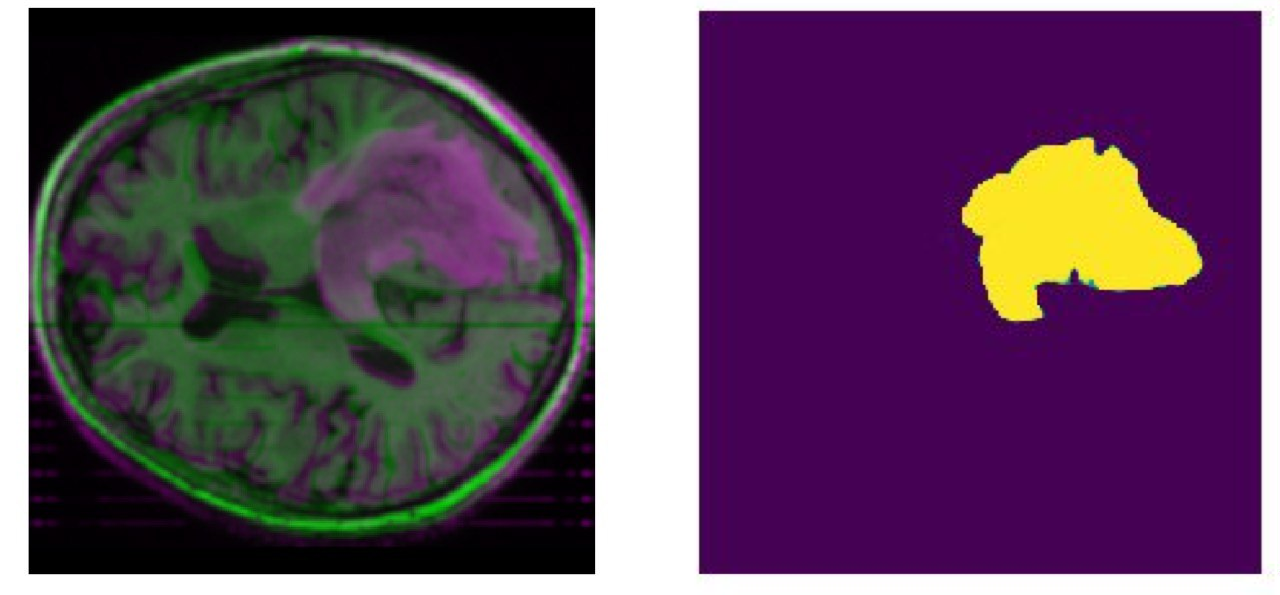
\includegraphics[width=\linewidth]{images/mri-sample.png}
\caption{Пример работы сети на изображении МРТ}\label{mri-sample}
\centering
\end{figure}



\section{Данные}

В качестве датасета использовался LIDC-IDRI \cite{lidc} - открытый набор данных в формате DICOM, размеченный 4-мя радиологами. Всего в датасете содержится 1018 сканов и более 7000 новообразований. Новообразование включалось в размеченное множество, если оно было выявлено хотя бы одним из специалистов.


\section{Детали реализации}

\subsection{Обучение}

Изначально планировалось подавать на вход сети полные 2D изображения для того, чтобы сеть смогла получить эффективное представление признаков изображений и выявить характерные свойства пространственного расположения опухолей. Однако результат данного подхода был отрицательный, поскольку сеть была не в состоянии обучиться и функция потерь не уменьшалась. Попытки использовать другую архитектуру Unet сети и изменить функцию потерь на функцию Focal Loss, отдающую предпочтение ложно положительным пикселям нежели ложно-отрицательным, не привели к успеху. Неудачу также потерпела попытка уменьшить количество данных в обучающем множестве убрав двухмерные изображения, не содержащие опухоли вообще, которых было более 80\%.

Подобное поведение сети скорее всего объясняется тем, что градиентный спуск застрявает в локальном минимуме, который соответствует тому, что сеть выдает пустые изображения, поскольку площадь маски очень мала по сравнению с изображеним.

Чтобы решить данную проблемы было предложено подавать сети не полные изображения, а их обрезанные куски. Изображение делилось сеткой на $n^2$ равных частей, из которых выбирались две части - содержащая опухоль и не содержащая. Далее эти части подавались на вход сети. При $n = 8$ сеть все еще не могла обучиться, но при $n = 16$ удалось получить результат.

\subsection{Тестирование}

Поскольку адекватный результат сеть выдавала только на маленьких обрезанных кусках изображения, для тестирования была использована следующая стратегия:

\begin{enumerate}
    \item Изображение делилось сеткой на $16^2$ частей
    \item Каждая часть независимо подавалась на вход сети
    \item Выходы сети склеивались для получения итоговой маски
    \item Так как выход сети представляет из себя двумерный массив пикселей, где значение каждого пикселя является действительным числом, вручную выбирается некоторый порог $0 < t < 1$
    \item Все пиксели имеющие значение, большее $t$, считаются пикселями маски, остальные пиксели зануляются
\end{enumerate}



\section{Подсчет метрик качества}

Основным показателем соответствия между истинной и предсказанной маской был выбран коэффициент Дайса

$$ dice(y_{true}, y_{pred}) = \dfrac{2|y_{true} \cap y_{pred}|}{ |y_{true}| + |y_{pred}|} $$

Если модель выдавала пустую маску, и при этом в реальности на изображении не было патологий, коэффициент Дайса полагался равным $1$. Ниже приведены коэффициенты Дайса, усредненные по тестовой выборке для различных значений порога $t$ 

В качестве примера таблицы приведена таблица~\ref{tab1}.

\begin{table}[!h]
\caption{Таблица умножения (фрагмент)}\label{tab1}
\centering
\begin{tabular}{|*{18}{c|}}\hline
\textbf{Порог $t$} & \textbf{Коэффициент Дайса} \\\hline
0.4 & 0.15 \\\hline
0.45 & 0.08 \\\hline
0.5 & 0.1 \\\hline
\end{tabular}
\end{table}

\section{Визуальный анализ}

\begin{figure}[!h]
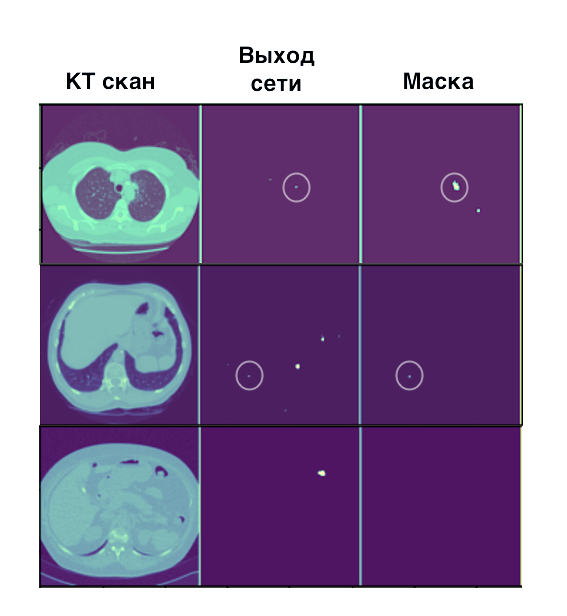
\includegraphics[width=\linewidth]{images/2d-seg-results.png}
\caption{Результаты работы сети}\label{mirskiy-cgan-architecture}
\centering
\end{figure}

Кругом обозначены совпадения на выходе сети и на истинной маске. На нижнем примере видно, что сеть ошибочно распознала участок ткани визуально похожий на опухоль, но в реальности ею не являющийся.

\section{Выводы по главе 2}

Полученные результаты явно свидетельствуют о непригодности использования подобных $end-to-end$ технологий для сегментации $2d$ изображений. Предполагаемое объяснение состоит в том, что двухмерные сканы не в состоянии передать достаточный набор признаков, позволяющий отличить опухоль от другого, похожего на нее участка легкого. Дело в том, что каждый двухмерный слайс содержит только лишь срез трехмерной опухоли, и значительная часть таких срезов может иметь вполне неопределенную форму, ничем не отличимую от сосудов в легких. Отсюда следует большая необходимость в использовании трехмерных зависимостей между различными слайсами для решения задачи распознавания.



\chapter{Описание предлагаемого подхода для 3D локализации}

В этой главе будет описано предлагаемое решение задачи 3D локализации новообразований по снимкам КТ легких.

\section{Модель локализации опухолей}

Для детекции опухолей была заимстована сверточная сеть с архитектурой Squeeze and Excitation Encoder Decoder \cite{li2019deepseed}. Сеть использует архитектуру ResNet18 в качестве кодировщика со встроенными SE модулями после каждого сверточного блока ResNet (остаточного блока). 

Структуру кодировщика отражает декодирощик, слои которого связаны skip-соединениями с кодировщиком. Выход декодирвщика подается на вход Region Proposal Network (RPN), задачей которой является предсказание координат различных bounding box-ов и вероятностей того, что в том или ином bounding box-е заключено новообразование.

\begin{figure}[!h]
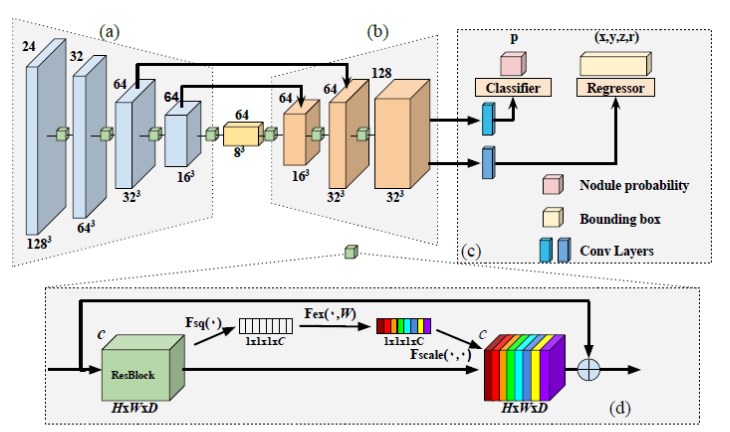
\includegraphics[width=\linewidth]{images/deep-seed-architecture.png}
\caption{Архитектура используемой сети DeepSEED}\label{deep-seed-architecture}
\centering
\end{figure}


\section{Аугментация данных с помощью генеративных противоборствующих сетей}

Широко известно применение генератиных противоборствующих сетей для генерации данных, которые впоследствии могут быть использованы в качестве расширения существующего датасета, на котором предполагается обучать детектор. В ряде работ были проведены визуальные тесты Тьюринга, где радиологам было предложено попробовать отличить генерированные опухоли от оригинальных. Специалисты не очень хорошо справились с задачей, что может говорить о том, что сети способны генерировать достаточно хорошие изображения, чтобы их можно было использовать в обучающем множестве.

\subsection{Модель генеративной противоборствующей сети}

Для решения данной задачи было принято решение заимствовать сеть, предложенную в работе \cite{mirsky}. У данной статьи есть документированная и удобная реализация в открытом доступе, в которой реализованы два фреймворка - один предназначен для добавления генерированных опухолей на изображение, второй предназначем для удаления опухолей с изображения. Для задачи аугментации данных естественно позаимствовать первый фреймворк который помимо реализации непосредственно архитектуры сети, предоставляет еще и возможность предобработки данных, которая состоит из нормализации и гистограммного выравнивания изображений.

Модель построена на условных GAN (Conditional GAN, CGAN), и основной задачей генератора является создание правдоподобной опухоли из некоторого шума и контекста. Сеть получает на вход $x_r^*$ - участок КТ изображения размера $32^3$, содержащий опухоль, из которого вырезан центральный куб размера $16^3$, и на его место вставлена маска из нулей. Оставшаяся часть участка $x_r^*$ выступает в роли контекстного окружения. Сеть генератора состоит из нескольких сверточных слоев (кодировщика) и нескольких декодирующих слоев, которые соединены с кодирующими слоями попарно (skip connection). После каждого сверточного блока применяется батчевая нормализация. Выход генератора - $G(x_r^*, \theta_g)$ наряду с оригинальным участком изображения $x_r$ далее подаются на вход дискриминатору, задачей которого является классифицировать объекты как оригинальные или генерированные.

\begin{figure}[!h]
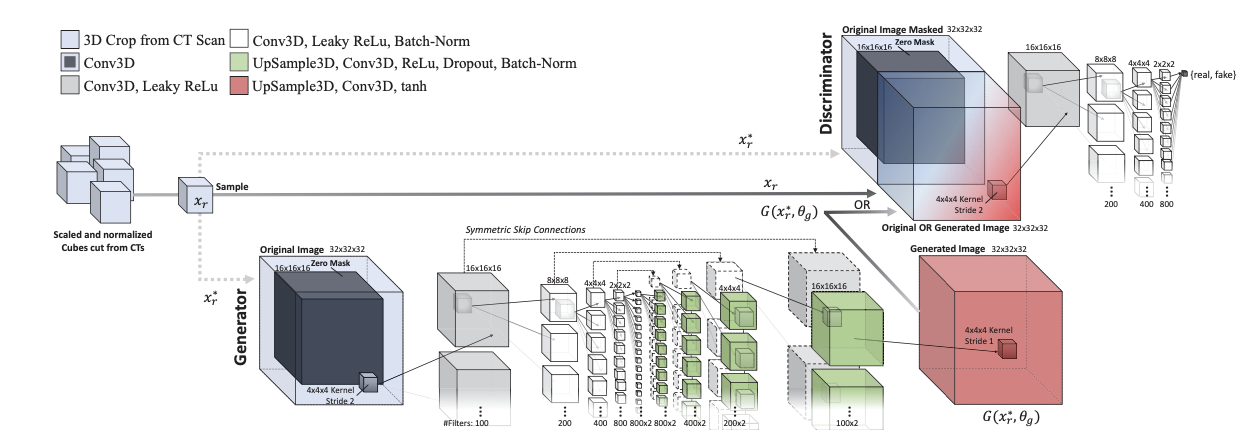
\includegraphics[width=\linewidth]{images/mirskiy-cgan-architecture.png}
\caption{Архитектура используемой сети CGAN}\label{mirskiy-cgan-architecture}
\centering
\end{figure}

\subsection{Адаптивная нормализация объектов (AdaIN)}

Адаптивная нормализация является популярной технологией и служит альтернативой батчевой нормализации и объектной нормализации, применяемой после каждого сверточного блока. Поэтому для совершенствования генеративной сети было предложено использовать ее вместо батчевой нормализации для эффективного и обучаемого преобразования промежуточных данных.

Адаптивная нормализация применяется следующим образом: Тензором $x$ принимается на вход. Размерности тензора: 

$$(b, xdim, ydim, zdim, c)$$, где $b$ - количество объектов в батче, $c$ - количество каналов, $xdim, ydim, zdim$ - пространственные размерности сооответственно.

нормализуется по все пространственным измерениям, то есть это происходит независимо для каждого канала и объекта в отличие от батчевой нормализации и аналогично объектной нормализации (Instance Normalization). Параметры афинного преобразования имеют размерность 

$$(b, 1, 1, 1, c)$$

То есть данные параметры аналогично варьируются по каналам и объектам.

\section{Итоговая процедура обучения}

В результате предложенная процедура обучения имеет следующий вид:

\begin{enumerate}
    \item Из датасета КТ изображений легких выбираются те, которые удовлетворяют некоторым ограничениям и соответственно являются пригодными для обучения CGAN
    \item Из выбранных данных вырезанются участки, содержащие опухоль, для создания объектов, которые можно непосредственно подать на вход CGAN.
    \item Данные аугментируются стандартными способами (повороты, отражения)
    \item Данные проходят предобработку: гистограммное выравнивание и нормализацию
    \item Данные, снабженные шумом на месте опухоли и окружающим контекстом подаются на вход CGAN для обучения
    \item Сеть CGAN, натренированная генерировать опухоли получает на вход предобработанные контексты для непосредственной генерации
    \item Данные, полученные на выходе CGAN, дополняют оригинальный датасет
    \item Сеть DeepSEED обучается на дополненном датасете.
\end{enumerate}



\chapter{Результаты решения задачи 3D локализации}

\section{Используемые данные}

В качестве датасета использовался не LIDC-IDRI непосредственно, как это было сделано в решении задачи 2d-сегментации, а его подможество LUNA \cite{luna}, содержащее 888 сканов в формате MetalImage и 1187 опухолей, каждая из которых представленна в виде bounding box. В отличие от LIDC-IDRI из LUNA исключены сканы, по толщине превосходящие 2.5 мм, а также включены только те опухоли, которые были размечены хотя бы тремя и четырех специалистов-радиологов. Еще одна особенность LUNA по сравнению с LIDC состоит в том, что средний размер новообразований в LUNA составляет 8.3 мм при стандартном отклонении в 4.8 мм, когда для LIDC-IDRI эти показатели составляют 12.8мм и 10.6 мм соответствено.

\section{Детали реализации}

\subsection{Реализация DeepSEED}

В оригинальной работе было предложено подавать на вход сети обрезанные участки КТ изображений размера $128^3$, однако такая размерность входных данный требует вычислительных ресурсов, которые были недоступны во время реализации, что привело к уменьшению размерности входа до $64^3$.


\subsection{Реализация Адаптивной нормализации}

Адаптивная нормализация была добавлена в сеть вместо батчевой нормализации. Она применяется после всех блоков (свертка, активация) и в кодировщике, и в декодировщике кроме первого слоя. В качестве входа $x$ формулы \eqref{eq:adain} используется тензор, полученный на выходе активации, а в качестве параметра $y$ используется выход побочной сети, имеющей простую архитектуру - 3 полносвязных слоя, причем первые два разделены между всеми побочными сетями. Данная архитектура позволяет выявить эффективные параметры афинного преобразования посредством обучения.

\subsection{Реализация CGAN}

Изначально архитектура CGAN, формат и размерность входных и выходных данных были полностью заимствованы у авторов \cite{mirsky} в качестве бейслайн решения. Отметим, что при обучении генератора авторы использовали не стандартную функцию потерь, а комбинированную:

\begin{equation}
L(o, g, D_{output}, labels) = MSE(o, g) + MAE(o, g) + L_{G}(D_{output}, labels)
\end{equation}

$o, g$ - оригинальное и генерированное изображения, соответствующие одному контексту.

$L_{GAN}$ - это стандартная функция потерь генератора, рассчитываемая на выходах дискриминатора и реальных метках объектов. Посредством уменьшения данной функции потерь генератор непосредственно стремится обмануть диксриминатор. Однако наряду с этим авторы предлагают использовать функцию потерь, минимизирующую различия между оригинальными изображениями и генерированными.

Я обучил несколько моделей с полностью заимствованными параметрами, но во время обучения и оценки результатов было обнаружено несоклько проблем:

\begin{enumerate}
    \item Функция потерь дискриминатора оптимизировалась гораздо лучше, чем функция потерь генератора, и начиная с некоторой эпохи, дискриминатор почти всегда отличал генерированные изображения от оригинальных.
    
    \item Выходные изображения были достаточно четкими в области контекста, однако в области латентного входа, где предполагалось генерировать непосредственно опухоль, изображения были мутные.
    
    \item Некоторые модели генерировали очень похожие результаты на различных входах. Данная проблема известна как mode collapse.
\end{enumerate}

Для борьбы с данными проблемами было предпринято несколько различных модификаций сети

\begin{enumerate}
    \item Вариация соотношения числа обновлений генератора и дискриминатора
    \item Увеличение размерности входа 
    \item Вариация функции потерь
\end{enumerate}

\subsubsection{Вариация соотношения числа обновлений генератора и дискриминатора}

Данный подход является стандартным для решения ситуации, когда либо генератор, либо дискриминатор отстает от другого и обучается существенно медленнее, либо совсем не обучается, и функция потерь даже возрастает. В моделях бейслайн архитектуры функции потерь и генератора и дискриминатора уменьшались, однако точность дискриминатора достигала 100\% и далее не уменьшалась. Несмотря на то, что генератору не удавалось обмануть дискриминатор, обучениие продолжало происходить в связи с присутствием $MSE$ и $MAE$ компонент. Данный подход кажется неудовлетворительным, поскольку в таком случае роль дискриминатора фактически отпадает и генератор просто стремится произвести похожее на оригинал изображение.

При увеличении соотношения числа обновлений с $1:1$ до $10:1$ в пользу генератора удалось получить визуально лучшие результаты


\section{Результаты}

\subsection{Результаты локализации с помощью DeepSEED}

В качестве метрик качества были выбраны ROC и FROC кривые. Стоит отметить, что FROC-анализ является достаточно популярным в области локализации новообразований легких. FROC-кривая аналогична ROC-кривой, но по оси $x$ отмечен не процент ложно положительных результатов, а среднее количество ложно-положительных bounding-box-ов на один скан.

Для визуализации результатов на рисунках \ref{roc-baseline} и \ref{froc-baseline} предоставлены графики, полученные в результате тестирования обученной модели.

\begin{figure}[!h]
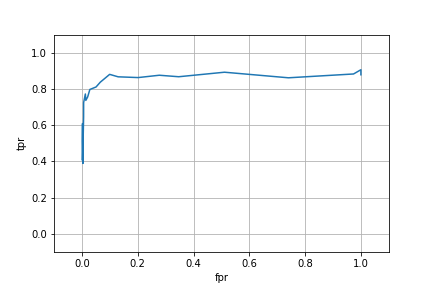
\includegraphics[width=\linewidth]{images/roc.png}
\caption{ROC результаты}\label{roc-baseline}
\centering
\end{figure}

\begin{figure}[!h]
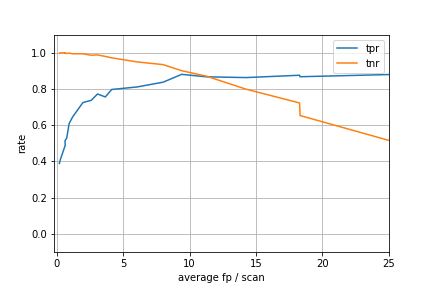
\includegraphics[width=\linewidth]{images/froc.png}
\caption{FROC результаты}\label{froc-baseline}
\centering
\end{figure}

Интересно также сравнить FROC кривые полученные нами и авторами оригинальной статьи. На рисунке \ref{froc-lifan} приведена FROC-кривая из оригинальной статьи.

\begin{figure}[!h]
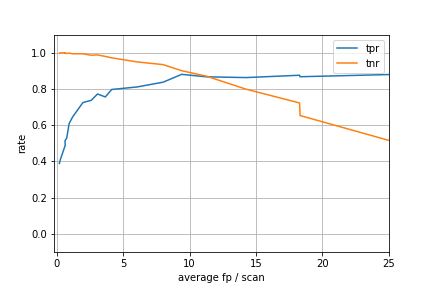
\includegraphics[width=\linewidth]{images/froc.png}
\caption{FROC-результаты (Li, Fan)}\label{froc-lifan}
\centering
\end{figure}

Стоит отметить схожесть кривых. Полученные результаты оказались несколько хуже результатов в статье, что возможно объяснить вынужденным сокращением размерностей обрезанных изображений, подаваемых на вход DeepSEED.

\subsection{Результаты обучения CGAN}

Для оценки качеcтва работы сети CGAN в первую очередь применялся визуальный анализ. На рисунке \ref{mirskiy-results} представлены примеры генерированных изображений, заимствованные из работы Мирского и др. На рисунке \ref{cgan-baseline-results} представлены результаты работы CGAN, предложенной в статье, но обученной нами. На рисунке \ref{cgan-adain-results} представлены результаты работы CGAN, в архитектуру которого вместо BN добавлен AdaIN

\begin{figure}[!h]
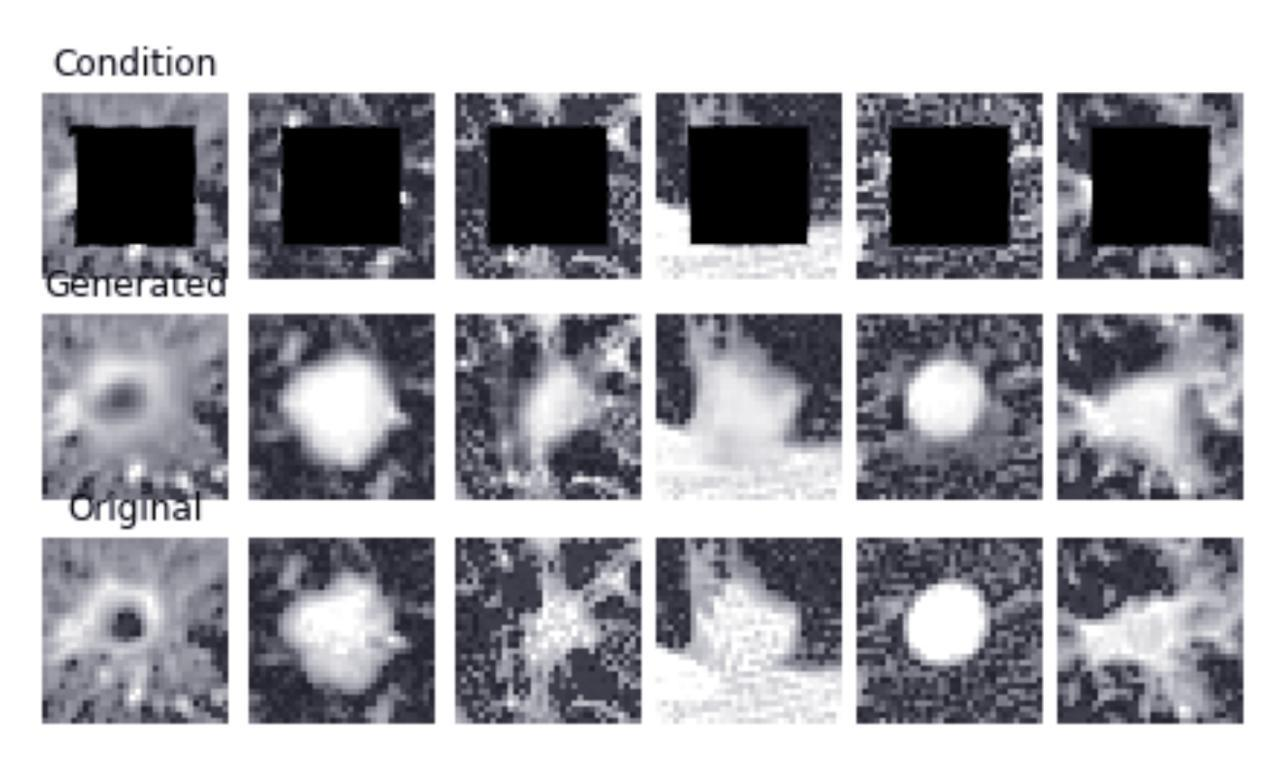
\includegraphics[width=\linewidth]{images/mirskiy-results.jpg}
\caption{Пример генерированных изображений (Mirsky et.al.)}\label{mirskiy-results}
\centering
\end{figure}

\begin{figure}[!h]
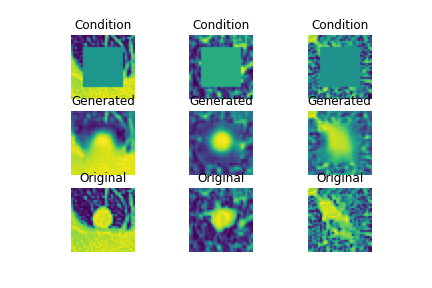
\includegraphics[width=\linewidth]{images/no-adain.png}
\caption{Пример генерированных изображений (Без AdaIN)}\label{cgan-baseline-results}
\centering
\end{figure}

\begin{figure}[!h]
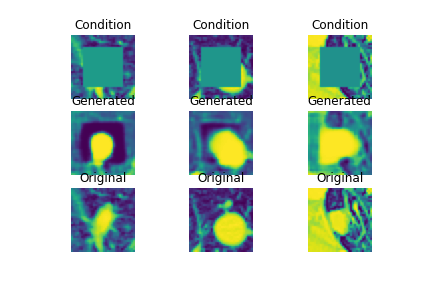
\includegraphics[width=\linewidth]{images/adain.png}
\caption{Пример генерированных изображений (С использованием AdaIN)}\label{cgan-adain-results}
\centering
\end{figure}

\section{Выводы}

\begin{figure}[!h]
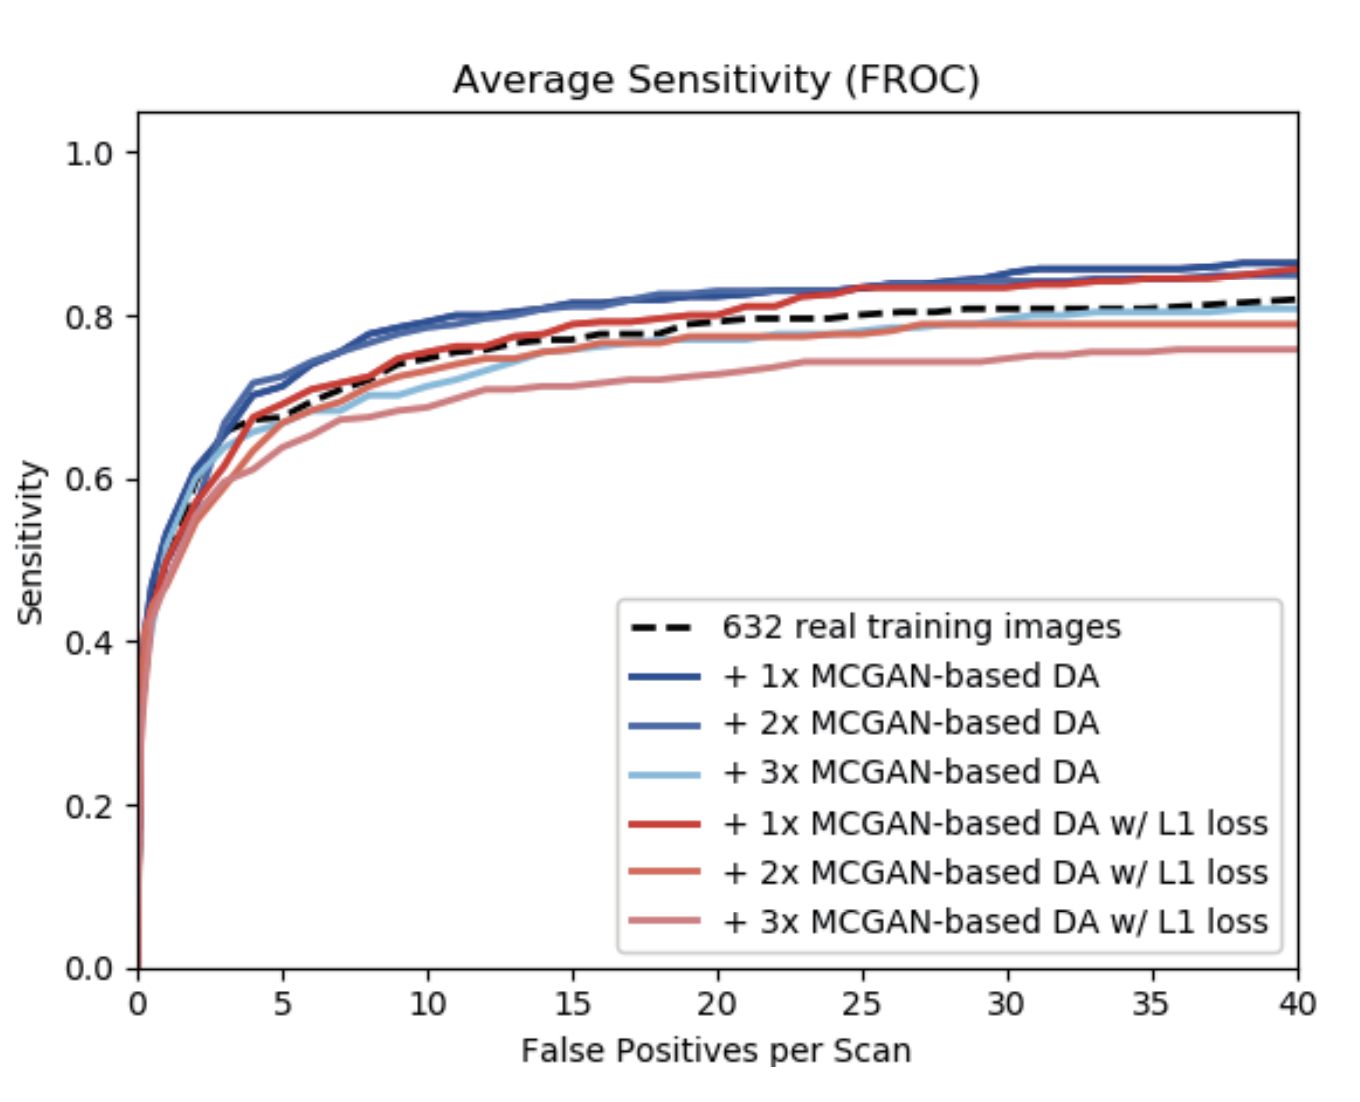
\includegraphics[width=\linewidth]{images/mcgan-results.png}
\caption{MCGAN FROC, Han et al. \cite{mcgan-augmentation}}\label{mcgan}
\centering
\end{figure}


\section{Применимость полученных методов на современных данных}

\printmainbibliography

\appendix

\chapter{Графики FROC метрик}\label{sec:app:1}

В данном приложении приведены пять графиков FROC-метрик для сравнительного ананлиза бейслайн решения и предложенной модификации с аугментацией. Каждый график соответствует одному эксперименту из таблицы \ref{tab:result-metrics}

\begin{figure}[!h]
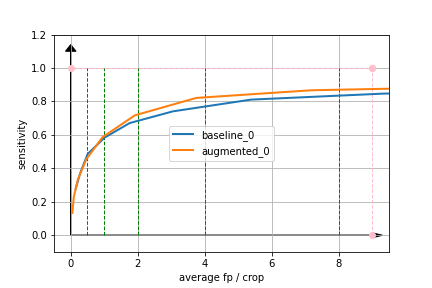
\includegraphics[width=\linewidth]{images/froc-results/cv_plot_0.png}
\caption{Итоговые FROC (over crop) кривые}\label{image:final-results-0}
\centering
\end{figure}

\begin{figure}[!h]
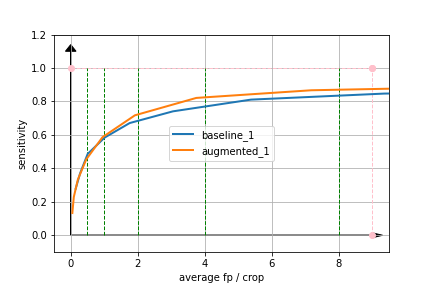
\includegraphics[width=\linewidth]{images/froc-results/cv_plot_1.png}
\caption{Итоговые FROC (over crop) кривые}\label{image:final-results-1}
\centering
\end{figure}

\begin{figure}[!h]
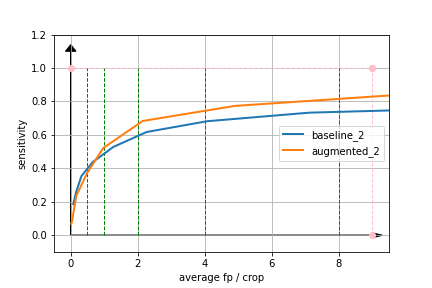
\includegraphics[width=\linewidth]{images/froc-results/cv_plot_2.png}
\caption{Итоговые FROC (over crop) кривые}\label{image:final-results-2}
\centering
\end{figure}

\begin{figure}[!h]
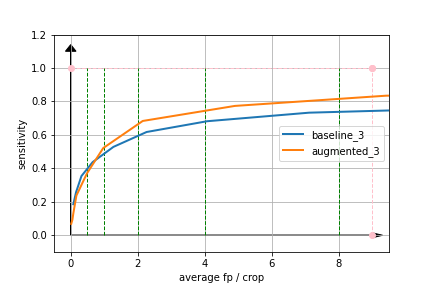
\includegraphics[width=\linewidth]{images/froc-results/cv_plot_3.png}
\caption{Итоговые FROC (over crop) кривые}\label{image:final-results-3}
\centering
\end{figure}

\begin{figure}[!h]
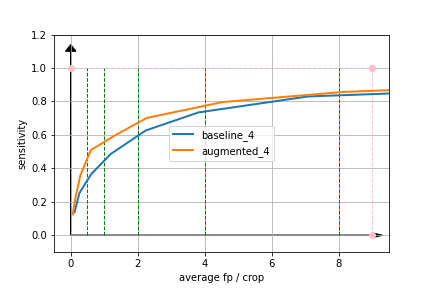
\includegraphics[width=\linewidth]{images/froc-results/cv_plot_4.png}
\caption{Итоговые FROC (over crop) кривые}\label{image:final-results-4}
\centering
\end{figure}

\end{document}